% Based on Diagram of Android activity life cycle
\documentclass[border=10pt]{standalone}
\usepackage{tikz}
\usetikzlibrary{arrows.meta,shapes, calc}
\tikzset{%
  >={Latex[width=2mm,length=2mm]},
  % Specifications for style of nodes:
            base/.style = {rectangle, rounded corners, draw=black,
                           minimum width=4cm, minimum height=1.5cm,
                           text centered, font=\sffamily},
  separateModel/.style = {base, fill=blue!20},
    internalIter/.style = {base, fill=green!20},
         process/.style = {base, minimum width=2.5cm, fill=orange!15},
         test/.style={process, diamond, aspect=2},
}
\begin{document}    
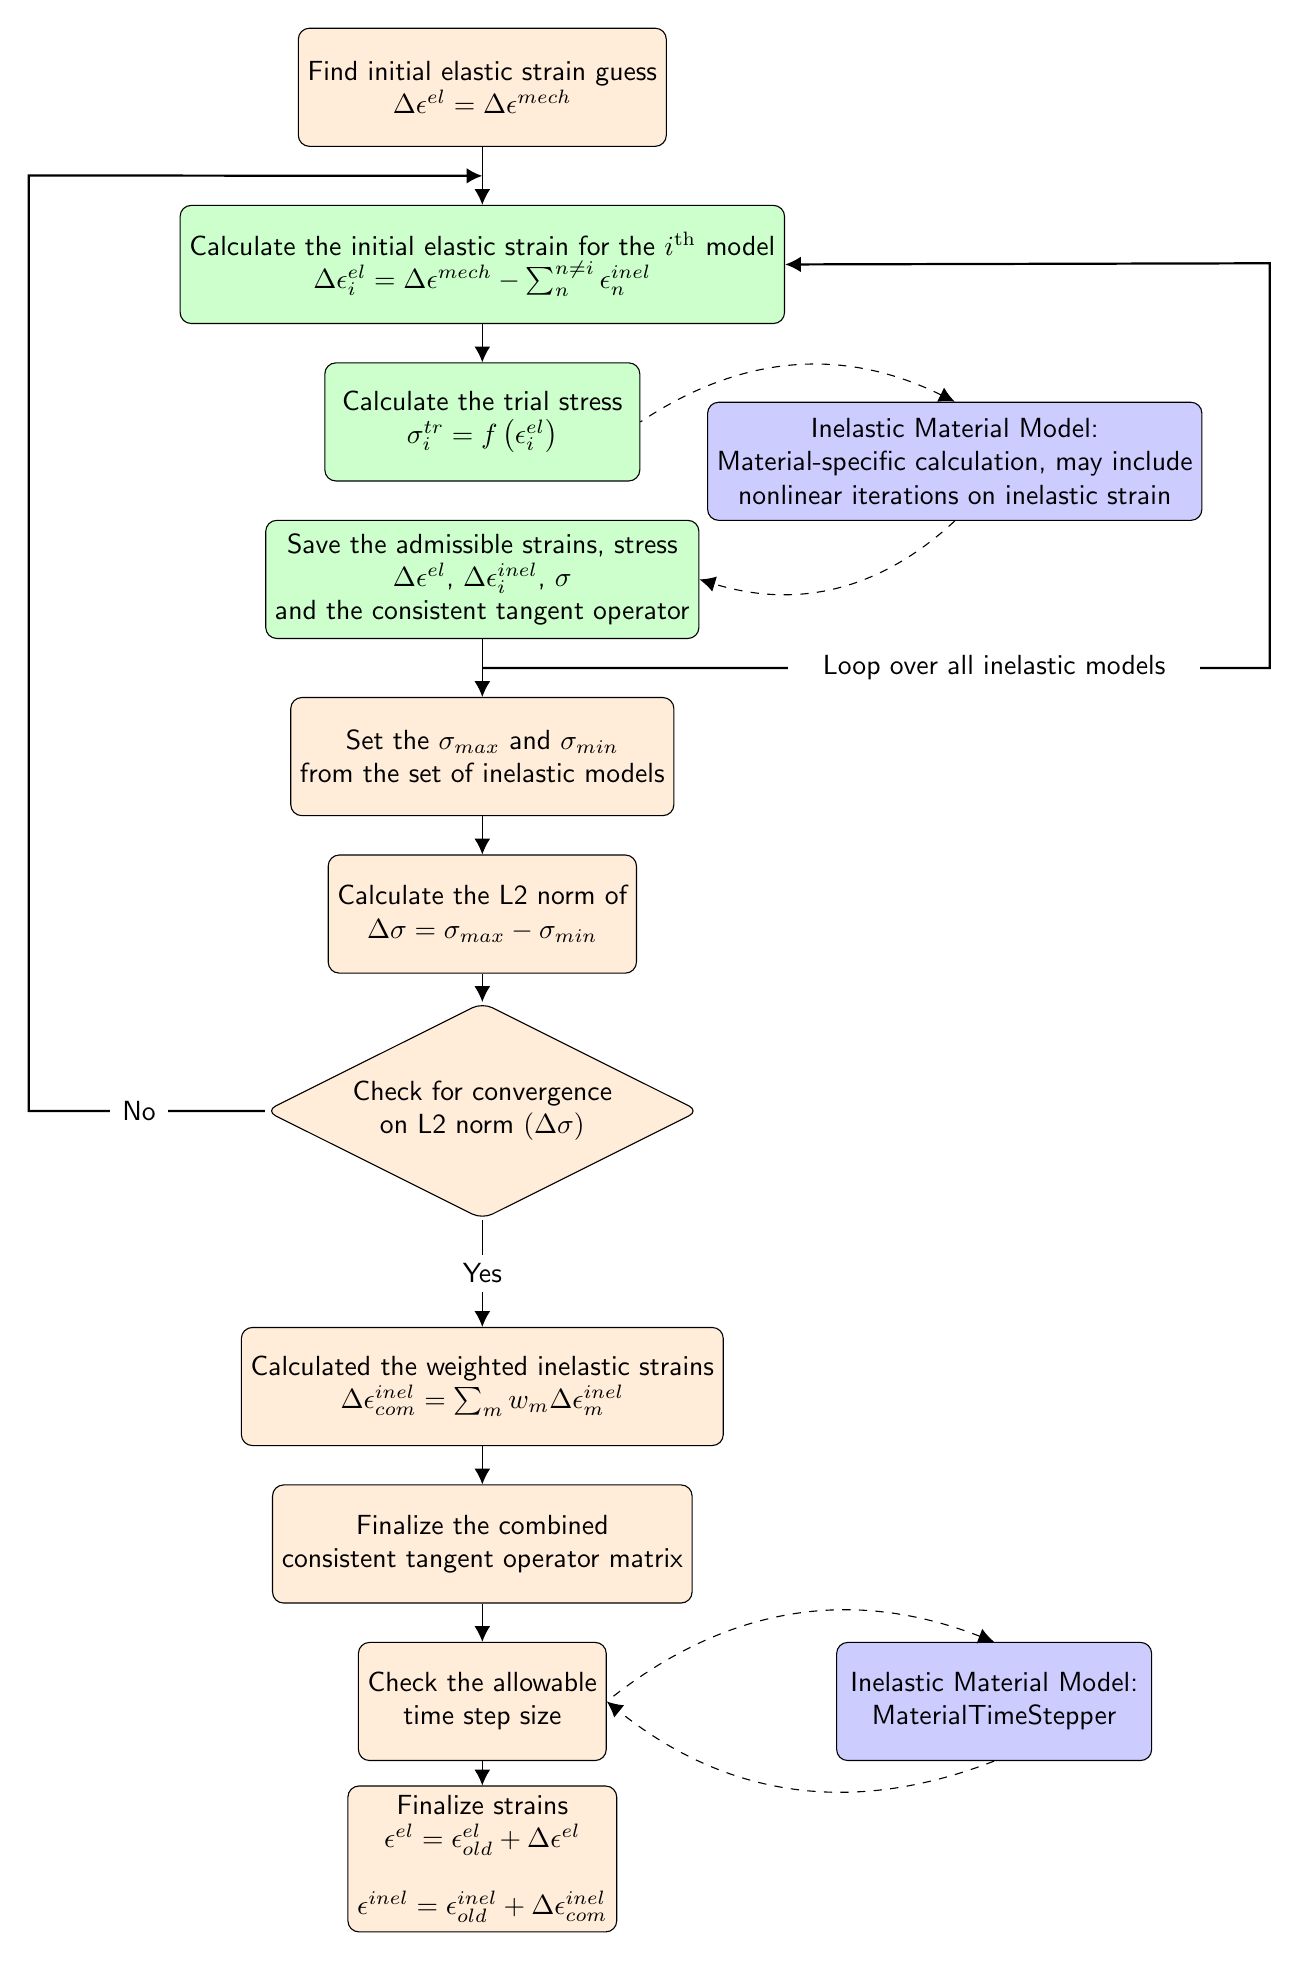
\begin{tikzpicture}[node distance=1.5cm,
    every node/.style={fill=white, font=\sffamily}, align=center]
  \node (start)               [process]
                              {Find initial elastic strain guess \\ $\Delta \epsilon^{el} = \Delta \epsilon^{mech}$};
  \node (initialStrainBlock) [internalIter, below of=start, yshift=-0.75cm]
                              {Calculate the initial elastic strain for the $i^{\mathrm{th}}$ model \\
                              $\Delta \epsilon^{el}_i = \Delta \epsilon^{mech} - \sum_n^{n \neq i} \epsilon^{inel}_n$};
  \node (trialStressBlock)    [internalIter, below of=initialStrainBlock, yshift=-0.5cm]
                              {Calculate the trial stress \\
                              $\sigma^{tr}_i = f \left( \epsilon^{el}_i \right)$};
  \node (matAdmissibleBlock)  [separateModel, right of=trialStressBlock, xshift=4.5cm, yshift=-0.5cm]
                              {Inelastic Material Model: \\ 
                               Material-specific calculation, may include \\ 
                               nonlinear iterations on inelastic strain};  
  \node (admissiblesBlock)    [internalIter, below of=trialStressBlock, yshift=-0.5cm]
                              {Save the admissible strains, stress \\
                              $\Delta \epsilon^{el}$, $\Delta \epsilon^{inel}_i$, $\sigma$\\
                              and the consistent tangent operator};                            


  \node (setStressBounds)     [process, below of=admissiblesBlock, yshift=-0.75cm]
                              {Set the $\sigma_{max}$ and $\sigma_{min}$ \\ from the set of inelastic models};
  \node (l2NormCalcBlock)     [process, below of=setStressBounds, yshift=-0.5cm]
                              {Calculate the L2 norm of \\ $\Delta \sigma = \sigma_{max} - \sigma_{min}$};
  \node (convergenceBlock)    [test, below of=l2NormCalcBlock,  yshift=-1cm]
                              {Check for convergence \\ on L2 norm $\left( \Delta \sigma \right)$};
  \node (weightedStrainBlock) [process, below of=convergenceBlock, yshift=-2cm]
                              {Calculated the weighted inelastic strains \\ $\Delta \epsilon^{inel}_{com} = \sum_m w_m \Delta \epsilon^{inel}_m $};
  \node (finalizeCTOBlock)    [process, below of=weightedStrainBlock, yshift=-0.5cm]
                              {Finalize the combined \\ consistent tangent operator matrix};
  \node (matTimeStepBlock)    [process, below of=finalizeCTOBlock, yshift=-0.5cm] 
                              {Check the allowable \\ time step size};
                              
  \node (materialTimeStepper) [separateModel, right of=matTimeStepBlock, xshift=5cm]
                              {Inelastic Material Model: \\ MaterialTimeStepper};
  \node (finalizeStrainBlock) [process, below of=matTimeStepBlock, yshift=-0.5cm] 
                              {Finalize strains \\
                              $\epsilon^{el} = \epsilon^{el}_{old} + \Delta \epsilon^{el}$ \\ 
                              \vspace{0.01cm} \\
                              $\epsilon^{inel} = \epsilon^{inel}_{old} + \Delta \epsilon^{inel}_{com}$};
 
  % Specification of lines between nodes specified above
  % with aditional nodes for description 
  \draw[->]                   (start) -- (initialStrainBlock);
  \draw[->]      (initialStrainBlock) to (trialStressBlock);

  \draw[<-, bend right=30, dashed] (matAdmissibleBlock.north) to (trialStressBlock.east);
  \draw[->, bend left=30, dashed]  (matAdmissibleBlock.south) to (admissiblesBlock.east);
  
  
  \draw[->]        (admissiblesBlock) to (setStressBounds);
  \draw[->]         (setStressBounds) -- (l2NormCalcBlock);
  \draw[->]         (l2NormCalcBlock) -- (convergenceBlock);
  \draw[->]        (convergenceBlock) -- node {Yes} (weightedStrainBlock);
  \draw[->]     (weightedStrainBlock) --  (finalizeCTOBlock);
  \draw[->]        (finalizeCTOBlock) -- (matTimeStepBlock);
  \draw[->]        (matTimeStepBlock) -- (finalizeStrainBlock);
  
  \draw[<-, bend right=30, dashed] (materialTimeStepper.north) to (matTimeStepBlock.east);
  \draw[->, bend left=30, dashed]  (materialTimeStepper.south) to (matTimeStepBlock.east);

  \draw[->, thick] ($(admissiblesBlock)!0.5!(setStressBounds)$) -- node[xshift=1.5cm, text width=5cm]{Loop over all inelastic models} ++(10,0) -- ++(0,5.14) --                
     (initialStrainBlock.east);

  \draw[->, thick] (convergenceBlock.west) -- node[xshift=-0.1cm, text width=0.5cm]{No} ++(-3,0) -- ++(0,11.88) --               
            ($(start)!0.5!(initialStrainBlock)$);
  \end{tikzpicture}
\end{document}